\documentclass[conference]{IEEEtran}
\IEEEoverridecommandlockouts
% ============================================================
%  Neuromarketing paper skeleton
%  Template: IEEEtran (conference, two-column)
%  See README.md in this folder for compilation instructions
%  and a guide to every TODO marker below.
% ============================================================

\usepackage{cite}
\usepackage{amsmath,amssymb,amsfonts}
\usepackage{graphicx}
\usepackage{textcomp}
\usepackage{xcolor}
\usepackage{booktabs}
\usepackage{multirow}
\usepackage{hyperref}
\usepackage{tikz}
\usetikzlibrary{shapes.geometric, arrows.meta, positioning, fit, backgrounds}
\usepackage{placeins}

% ---- TODO helper: makes every placeholder impossible to miss.
% Delete \TODO{...} calls once you replace them with real content;
% the paper should contain ZERO red text before you submit it.
\newcommand{\TODO}[1]{\textcolor{red}{\textbf{[TODO: #1]}}}
\newcommand{\TBD}{\textcolor{red}{\textbf{TBD}}}

\def\BibTeX{{\rm B\kern-.05em{\sc i\kern-.025em b}\kern-.08em
    T\kern-.1667em\lower.7ex\hbox{E}\kern-.125emX}}

\begin{document}
\pagestyle{plain}

\title{An End-to-End EEG-Based Neuromarketing Pipeline for\\
Emotion-Driven Advertising Optimization}

\author{
\IEEEauthorblockN{Onobiono Yakana Karl Jerry}
\IEEEauthorblockA{\textit{aivancity} \\ France}
\and
\IEEEauthorblockN{Florian Hounkpatin}
\IEEEauthorblockA{\textit{aivancity} \\ France}
\and
\IEEEauthorblockN{Ephraïm Kossonou}
\IEEEauthorblockA{\textit{aivancity} \\ France}
\and
\IEEEauthorblockN{Noemi Dombou}
\IEEEauthorblockA{\textit{aivancity} \\ France}
}

\maketitle
\thispagestyle{plain}

\begin{abstract}
Advertising effectiveness is traditionally assessed after the fact, through
recall surveys or click-through metrics that say little about the moment-to-moment
emotional experience of the viewer. This paper presents an
end-to-end pipeline that predicts a viewer's affective state,
valence and arousal, directly from electroencephalography (EEG) and
peripheral physiological signals, relates that predicted state to a
learned model of self-reported liking, and produces a quantified,
time-resolved gap report between the observed emotional trajectory and
an empirically optimal one. The gap report is then translated into
natural-language creative recommendations by a large language model
(LLM), closing the loop between neurophysiological measurement and
actionable advertising edits. We build and validate the pipeline on the
DEAP dataset~\cite{koelstra2012deap}, comparing classical machine
learning models (Random Forest, Gradient Boosting, Ridge regression)
against a convolutional neural network trained on multichannel EEG
spectrograms, under two cross-validation regimes, window-level
GroupKFold and video-level leave-one-video-out, chosen specifically
to avoid the temporal leakage that inflates reported accuracy in much of
the EEG-emotion literature. Across all classical models, window-level
$R^2$ is negative (e.g.\ $-0.47$ to $-3.1$ depending on model and target),
and the stricter video-level leave-one-video-out metric sits at or below a
mean-prediction baseline for both targets (best result: $R^2 = 0.01$ for
arousal with Random Forest), confirming that within-subject
valence/arousal prediction from this feature set is weak on DEAP.
Pooling windows across all 32 subjects and normalizing each subject's own
feature scale stabilizes an otherwise unstable Ridge baseline but does
not produce genuine unseen-subject generalization, and a naive high/low
classification reframing that appears to reach 78\% accuracy is shown to
be an artifact of class imbalance, dropping to a near-chance 50-56\% once
classes are rebalanced per subject. The LLM advisor stage was exercised
end to end with a live, locally hosted model on a real DEAP stimulus,
producing coherent, gap-grounded editorial recommendations; a systematic
evaluation across prompts, models, and a human-expert judgment of
recommendation quality, together with a full closed-loop trial on a
re-edited advertisement, remain future work.
\end{abstract}

\begin{IEEEkeywords}
affective computing, EEG, neuromarketing, valence-arousal, DEAP dataset,
convolutional neural network, large language models, advertising optimization
\end{IEEEkeywords}

% =================================================================
\section{Introduction}
% =================================================================

Marketers have long relied on self-report (surveys, focus groups, recall
tests) to judge whether an advertisement ``worked.'' These instruments are
retrospective, coarse, and subject to well-documented biases: viewers
rationalize their reactions after the fact and struggle to report the
fine-grained emotional dynamics that actually determine whether an ad is
remembered, shared, or ignored~\cite{lee2007neuromarketing}. Physiological
signals (EEG, galvanic skin response, heart rate, muscle activity)
offer a complementary, involuntary channel: they change on the timescale of
seconds, well before a viewer could consciously articulate a preference,
and they are difficult to fake.

The scientific basis for turning these signals into something actionable is
the circumplex model of affect~\cite{russell1980circumplex}, which
represents any emotional state as a point in a two-dimensional space of
\emph{valence} (how positive or negative the experience is) and
\emph{arousal} (how activating or calming it is). If valence and arousal
can be estimated continuously from physiological signals, and if the
combination of valence and arousal that maximizes \emph{liking} for a given
audience is known, then the distance between what a viewer is actually
feeling and what they would ideally be feeling becomes a measurable,
optimizable quantity.

This paper describes a system that operationalizes that idea
end to end:

\begin{enumerate}
\item \textbf{Signal-to-affect}: EEG and peripheral signals are converted
into an 85-dimensional feature vector per 2-second window and mapped to
predicted valence and arousal, $(\hat V, \hat A)$, using either classical
regressors on hand-crafted spectral features or a convolutional neural
network (CNN) trained on multichannel time-frequency spectrograms.
\item \textbf{Affect-to-liking}: a response surface
$g(V, A) \rightarrow \text{Liking}$ is fit on the DEAP self-report labels
and used to locate the \emph{optimal zone} $(V^{*}, A^{*})$ that empirically
maximizes liking.
\item \textbf{Gap analysis}: the discrepancy between $(\hat V, \hat A)$ and
$(V^{*}, A^{*})$ is quantified per time segment, identifying exactly which
moments of an advertisement under-perform and along which dimension.
\item \textbf{LLM-based creative advisor}: the structured gap report,
combined with a text description of the advertisement, is passed to a
pretrained language model that proposes concrete editorial changes (pacing,
color palette, music, cuts) to move the predicted response toward the
optimal zone.
\item \textbf{Closed loop}: after an advertisement is re-edited, the same
pipeline re-measures it, allowing the recommendation to be evaluated
objectively by comparing the gap before and after.
\end{enumerate}

A central methodological concern of this work, discussed at length in
Section~\ref{sec:methodology}, is evaluation honesty. DEAP provides a
single self-reported label per one-minute video, which means that hundreds
of highly overlapping 2-second windows drawn from the same video share one
target. A naive window-level random split leaks information from a video's
test windows into its train windows and produces inflated, uninformative
accuracy. We instead report results under both a window-level
\texttt{GroupKFold} split, grouped by video, and a stricter video-level
\texttt{Leave-One-Video-Out} (LOVO) split, and treat the latter as the
scientifically meaningful number.

\textbf{Contributions.} (i) A complete, reproducible pipeline from raw EEG
to natural-language creative advice, implemented as an open Python
package~\cite{sourcecoderepo}; (ii) an explicit comparison of classical spectral-feature models
against a spectrogram-based CNN under leakage-safe evaluation; (iii) a
learned liking response surface used to define an interpretable,
per-segment optimization target for advertising content; (iv) a worked
demonstration of how an LLM can consume a purely numerical affective
report, with no access to the video itself, and produce plausible,
targeted creative recommendations.

The remainder of this paper is organized as follows. Section~\ref{sec:related}
reviews related work in EEG-based emotion recognition and neuromarketing.
Section~\ref{sec:data} describes the DEAP dataset. Section~\ref{sec:methodology}
details every stage of the pipeline. Section~\ref{sec:experiments} describes
the experimental protocol, Section~\ref{sec:results} reports results, and
Section~\ref{sec:discussion} discusses limitations before concluding in
Section~\ref{sec:conclusion}.

% =================================================================
\section{Related Work}
\label{sec:related}
% =================================================================

\subsection{EEG-based emotion recognition}
EEG-based affect recognition has been surveyed extensively; see
Alarc\~{a}o and Fonseca~\cite{alarcao2019emotions} for a comprehensive
overview of feature types, classifiers, and datasets used across the
field. Band-power features extracted with Welch's
method~\cite{welch1967psd} over the canonical EEG bands (theta, alpha,
low-beta, high-beta, gamma) remain a strong, interpretable baseline against
which deep architectures are usually compared. Recent work has pushed
substantially past hand-crafted band-power features on DEAP: Yao et
al.~\cite{yao2024transformercnn} combine parallel transformer encoders
(for spatial and temporal structure, respectively) with a CNN aggregation
head, reporting accuracies above 95\% for valence, arousal, and their
joint classification on DEAP, and similarly attention-augmented and
purely convolutional architectures have been reported in the
95-98\% range on the same benchmark. Two points about this literature are
worth stating plainly given how it contrasts with the results reported
here (Section~\ref{sec:results}). First, essentially all of these
figures are obtained under window-level, non-group-aware splits, exactly
the evaluation regime Section~\ref{subsec:splits} argues is
leakage-prone; classification accuracy in the mid-to-high 90s on a
task where each 60-second video is chopped into hundreds of
highly overlapping windows sharing one label is consistent with a model
partly recognizing near-duplicate training neighbors of each test window
rather than genuinely generalizing to unseen affective content, which is
precisely why this paper reports both window- and video-level (leave-one-
video-out) numbers rather than the former alone. Second, most of this
work targets discrete classification (typically high/low, sometimes 3-5
class), a substantially easier target than the continuous regression
pursued here; Section~\ref{sec:discussion} revisits this distinction once
our own classification-reframing results are reported.

\subsection{The DEAP dataset and evaluation leakage}
DEAP~\cite{koelstra2012deap} is one of the most widely used benchmarks in
affective computing, providing 32-channel EEG plus eight peripheral
channels recorded from 32 participants watching 40 one-minute music
videos, each rated on valence, arousal, dominance and liking. A
recurring methodological weakness in the literature, and the specific
issue this paper's evaluation protocol is designed to avoid, is
splitting overlapping windows from the same trial across train and test
sets, which produces near-perfect but scientifically meaningless accuracy.
We adopt group-aware and leave-one-video-out splits for this reason
(Section~\ref{subsec:splits}).

\subsection{Neuromarketing}
Neuromarketing applies neuroscientific measurement to marketing questions,
broadly defined by Lee et al.~\cite{lee2007neuromarketing} as ``the
application of neuroscientific methods to analyze and understand human
behaviour in relation to markets and marketing exchanges.'' Prior
neuromarketing work has largely stopped at \emph{measurement},
reporting which stimuli produce stronger engagement or more positive
affect, rather than closing the loop into \emph{actionable, automated}
creative recommendations. Yang et al.~\cite{yang2015tvcommercials}
directly evaluate TV commercials with neurophysiological responses,
relating EEG-derived engagement and frontal asymmetry measures to
subjective commercial ratings, while Raiesdana and
Mousakhani~\cite{raiesdana2022eegcar} use EEG to analyze consumer
preference toward an electric car advertisement, in both cases stopping
at a descriptive comparison of stimuli rather than generating a
prescriptive edit. This pattern is representative of the broader
literature: EEG (and other biosignals) are used to score or rank
existing creative variants after the fact, functionally replacing a
survey with a physiological measurement, but the measurement itself is
the end product, not one input to a subsequent recommendation step. The
gap analysis and LLM advisor stages of this paper
(Sections~\ref{subsec:gap}-\ref{subsec:advisor}) are aimed specifically
at that gap: turning a physiological measurement into a directional,
segment-level editorial recommendation rather than a single
engagement/liking score.

\subsection{LLMs as text-only creative advisors}
We searched specifically for prior work coupling a biosignal-derived
summary with a generative language model for content-editing guidance
and found none targeting advertising or affective content creation. The
closest related direction is recent work on LLMs consuming physiological
signals directly: Xie et al.~\cite{xie2025physllm} use an LLM to fuse
multimodal cues for remote photoplethysmography (camera-based heart-rate
estimation), which couples an LLM to a biosignal-adjacent task but
targets signal \emph{estimation}, not downstream creative
\emph{recommendation}, and operates on video/visual input rather than a
structured numerical report. To our knowledge, the specific design used
here, a text-only LLM that never observes the stimulus and receives only
a structured, quantitative gap report (Section~\ref{subsec:gap}) plus
externally supplied content metadata, and is asked to propose editorial
changes rather than to estimate or classify a signal, has not been
described elsewhere. We present this as a genuine gap rather than an
established sub-field, and flag it as the paper's most speculative
contribution: Section~\ref{subsec:advisor} demonstrates the architecture
end to end, but, as discussed in Section~\ref{sec:discussion}, without
yet an empirical evaluation of whether its output is judged useful by a
human advertising professional.

% =================================================================
\section{Dataset}
\label{sec:data}
% =================================================================

We use the DEAP dataset~\cite{koelstra2012deap}, comprising EEG (32
channels) and peripheral physiological signals (EOG, EMG, GSR,
respiration, blood volume pulse, skin temperature) from 32 subjects, each
watching 40 one-minute music-video excerpts. Each trial is labeled with
self-reported Valence, Arousal, Dominance and Liking on a continuous 1-9
scale. This work uses the pre-processed, downsampled (128\,Hz) version of
the dataset. Of the recorded channels, we retain the 14 EEG channels
matching the 10-20 system positions common to lower-cost consumer
headsets (for downstream applicability) and 8 peripheral channels; the
horizontal and vertical EOG channels are excluded as they capture ocular
artifacts rather than emotional signal.

One point worth making explicit, since the pipeline never touches the
video itself, only physiological signals: every time this paper refers to
``2 seconds'' or ``60 seconds'' of a trial, it means 2 or 60 seconds of
\emph{elapsed recording time}, not 2 or 60 seconds of video footage. While
a participant watched a video, their EEG and peripheral sensors recorded
continuously, on the same clock, at 128 samples every second, for exactly
as long as the video played. Because the recording and the video started
and stopped together, there is a precise, fixed correspondence between
elapsed video time and elapsed sample count: second $t$ of the video
corresponds to sample $\lfloor t \times 128 \rfloor$ of the signal,
regardless of what is happening on screen at that instant. So ``2 seconds
of data'' simply means 256 consecutive samples of that already-timestamped
recording (Section~\ref{subsec:features}); the pipeline knows precisely
\emph{when}, by timestamp, a participant's signal changed, but, since it
never sees the video's pixels or audio, has no notion of \emph{what} was
on screen at that moment unless that information is supplied separately
as text (Section~\ref{subsec:advisor}).

Every DEAP recording is actually 63 seconds long, not 60: the first 3
seconds are a \emph{pre-stimulus baseline}, during which the participant
looks at a blank fixation screen before the video begins. Because the
signal is sampled at 128\,Hz (128 measurements every second), those 3
seconds correspond to a fixed number of samples,
\begin{equation}
3\ \text{s} \times 128\ \tfrac{\text{samples}}{\text{s}} = 384\ \text{samples},
\label{eq:baseline}
\end{equation}
which is exactly the segment dropped from the start of every trial before
any feature is computed, leaving the 60-second, 7680-sample stimulus
period ($60 \times 128 = 7680$) used throughout the rest of this section.
DEAP's designers recorded this silent period so that each participant's
resting physiological state could be measured immediately before every
trial. The baseline period is never itself turned into a labeled training
window: during those 3 seconds the participant has not yet seen the
video, so windowing it would attach the trial's self-reported
$[\text{Valence}, \text{Arousal}]$ label to a signal that has nothing to
do with it, quietly teaching a model that a resting, pre-stimulus state
predicts the video's emotional response. This exclusion is unconditional
in every experiment reported here, including the per-subject window-level
and video-level (LOVO) results of Table~\ref{tab:window} and
Table~\ref{tab:lovo}, which use only the raw stimulus-period features
described in Section~\ref{subsec:features}.

Separately, as one of the cross-subject extensions of
Section~\ref{subsec:results-pooled}, we also evaluate a
\emph{baseline-corrected} variant of the features: the same
85-dimensional feature vector is additionally computed once over the
384-sample baseline itself, and this baseline vector is subtracted from
every stimulus window's feature vector for that trial, an attempt to
remove each participant's personal resting level (e.g.\ overall EEG power,
tonic skin conductance) so that only the change induced by the video
remains. We evaluate this correction empirically rather than assume it
helps, and, as Section~\ref{sec:results} reports, the outcome is mixed:
it made pooled window-level regression neutral-to-slightly-worse for most
models, while a separate, later fix (per-subject feature normalization)
stabilized an otherwise unstable cross-subject Ridge baseline
(Section~\ref{sec:discussion}), a more nuanced result than the
correction's motivation alone would predict.

% =================================================================
\section{Methodology}
\label{sec:methodology}
% =================================================================

Fig.~\ref{fig:pipeline} summarizes the full pipeline. The stages
summarized below run from raw signal to closed-loop re-measurement; this
section describes each in the order data flows through them.

\begin{figure*}[!t]
\centering
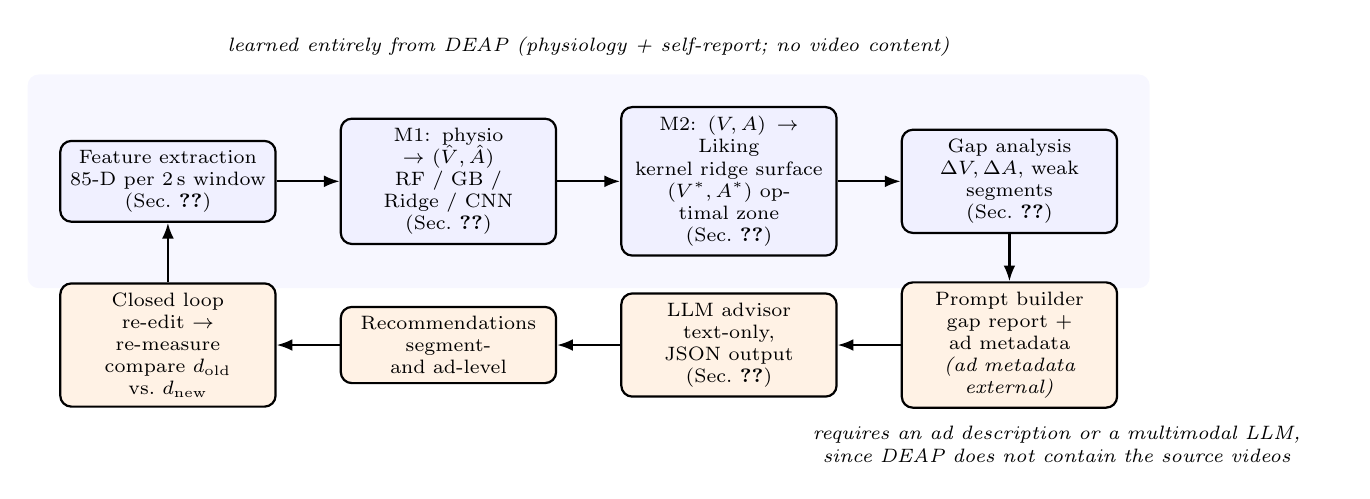
\begin{tikzpicture}[
  node distance = 6mm and 8mm,
  box/.style = {rectangle, draw, thick, rounded corners, align=center,
                minimum height=9mm, text width=25mm, font=\scriptsize, fill=blue!6},
  boxext/.style = {box, fill=orange!10},
  arr/.style = {-{Latex[length=2mm]}, thick}
]
  \node[box] (feat)  {Feature extraction\\85-D per 2\,s window\\(Sec.~\ref{subsec:features})};
  \node[box, right=of feat] (m1)   {M1: physio $\rightarrow$ $(\hat V,\hat A)$\\RF / GB / Ridge / CNN\\(Sec.~\ref{subsec:models})};
  \node[box, right=of m1]   (m2)   {M2: $(V,A)\rightarrow$ Liking\\kernel ridge surface\\$(V^{*},A^{*})$ optimal zone\\(Sec.~\ref{subsec:liking})};
  \node[box, right=of m2]   (gap)  {Gap analysis\\$\Delta V,\Delta A$, weak segments\\(Sec.~\ref{subsec:gap})};

  \node[boxext, below=of gap]  (prompt) {Prompt builder\\gap report + ad metadata\\\emph{(ad metadata external)}};
  \node[boxext, left=of prompt] (llm)   {LLM advisor\\text-only, JSON output\\(Sec.~\ref{subsec:advisor})};
  \node[boxext, left=of llm]    (rec)   {Recommendations\\segment- and ad-level};
  \node[boxext, left=of rec]    (loop)  {Closed loop\\re-edit $\rightarrow$ re-measure\\compare $d_{\text{old}}$ vs.\ $d_{\text{new}}$};

  \draw[arr] (feat) -- (m1);
  \draw[arr] (m1)   -- (m2);
  \draw[arr] (m2)   -- (gap);
  \draw[arr] (gap)  -- (prompt);
  \draw[arr] (prompt) -- (llm);
  \draw[arr] (llm)  -- (rec);
  \draw[arr] (rec)  -- (loop);
  \draw[arr] (loop.north) -- ++(0,4mm) -| (feat.south);

  \begin{scope}[on background layer]
    \node[fit=(feat)(m1)(m2)(gap), fill=blue!3, rounded corners, inner sep=4mm] (deapbox) {};
  \end{scope}
  \node[above=1mm of deapbox, font=\scriptsize\itshape] {learned entirely from DEAP (physiology + self-report; no video content)};
  \node[below=1mm of prompt, xshift=6mm, font=\scriptsize\itshape, text width=70mm, align=center]
       {requires an ad description or a multimodal LLM, since DEAP does not contain the source videos};
\end{tikzpicture}
\caption{The proposed pipeline. Blue boxes (top row) are trained and
validated entirely on DEAP signals and self-reports. Orange boxes (bottom
row) operate past the dataset boundary of Section~\ref{sec:data}: they
require an externally supplied advertisement description (or, in a
production system, a multimodal model with direct video access), since
DEAP itself contains no video content. The loop closes by re-measuring a
re-edited advertisement and feeding new physiological signals back into
feature extraction.}
\label{fig:pipeline}
\end{figure*}

\subsection{Feature extraction}
\label{subsec:features}

The 60-second, 7680-sample trial obtained above is not treated as one
long signal. Instead it is broken into many short snippets called
\emph{windows}, each analyzed separately. This is standard practice in
EEG analysis: the frequency content of brain activity changes too quickly
for a single power-spectrum estimate over 60 seconds to mean anything
useful, so features are instead computed on short segments over which the
signal can reasonably be treated as stable. Concretely, a window is
nothing more exotic than a fixed-length, contiguous slice of the sampled
signal, a (14 channels) $\times$ (256 samples) block of numbers for EEG,
an (8 channels) $\times$ (256 samples) block for peripheral signals, the
same way you might look at a long strip of film through a small moving
frame that only reveals a short stretch of it at a time.

This is also what \emph{window-level} computation means throughout the
rest of this paper: instead of computing one feature vector for an entire
60-second trial, which would give only 1 data point per trial (40 per
subject), each of the many windows extracted from a trial becomes its own
row of the dataset, $(X_i, y)$, where $X_i$ is the 85-dimensional feature
vector of window $i$ (70 EEG band-power values plus 15 peripheral
statistics, detailed below) and $y$ is the
trial's single self-reported $[\text{Valence}, \text{Arousal}]$ label.
Because DEAP provides only one label per 60-second trial, not one per
window, every window inherits the same label as its parent trial, a
deliberate simplification whose consequences (hundreds of rows sharing
one label) motivate the group-aware cross-validation protocol of
Section~\ref{subsec:splits} and the window-level/video-level distinction
used throughout the Results and Discussion.

Each window spans 256 samples, i.e.\ 2 seconds ($256 / 128\,\text{Hz} =
2\,\text{s}$), long enough for Welch's method (Section~\ref{subsec:models})
to produce a stable estimate of even the slowest band of interest (theta,
around 4-8\,Hz), while short enough to track emotional responses that can
shift within a few seconds. Rather than cutting the trial into 30
disjoint 2-second blocks, consecutive windows overlap: the start of the
window advances by a \emph{step} of 128 samples (1.0\,s) each time, not by
a full window length. Concretely, window 1 covers samples $[0, 256)$,
window 2 covers $[128, 384)$, window 3 covers $[256, 512)$, and so on, so
each new window shares $256 - 128 = 128$ of its 256 samples with the one
before it. As a fraction of the window length,

\begin{equation}
\text{overlap} = \frac{\text{window length} - \text{step}}{\text{window length}}
= \frac{256 - 128}{256} = 50\%,
\label{eq:overlap}
\end{equation}

\noindent which is where the 50\% figure comes from. \emph{This was not
the first configuration tried.} An earlier iteration of the pipeline used
a much finer step of 16 samples (0.125\,s, 93.75\% overlap), motivated by
two goals: more training rows per trial (465 windows/trial rather than the
59 used in the final configuration below), and finer temporal resolution
for the gap analysis of Section~\ref{subsec:gap} to localize weak segments
to a fraction of a second. In a direct controlled comparison on the same
subject and model (Random Forest, window-level GroupKFold), reducing the
overlap from 93.75\% to 50\% moved window-level $R^2$ for Valence from
$-0.480$ to $-0.393$ and for Arousal from $-0.200$ to $-0.127$, i.e.\ less
severely negative, consistent with the mechanism described below: at
93.75\% overlap, consecutive windows are near-duplicate copies of almost
the same signal, so a train/test split that is leakage-safe at the
\emph{video} level (Section~\ref{subsec:splits}) still lets the model
partially memorize highly correlated near-neighbors of each test window
sitting in the training fold, which is not information leakage in the
group-theoretic sense but does inflate how much genuinely new signal each
additional window contributes. We therefore report all results in this
paper under the 50\%-overlap, 1.0\,s-step configuration; the number of
windows per trial follows directly from the window length and step,

\begin{equation}
n_{\text{windows}} = \left\lfloor \frac{7680 - 256}{128} \right\rfloor + 1 = 59,
\label{eq:nwindows}
\end{equation}

\noindent an exact count: every one of the 40 trials, for every subject,
yields precisely 59 overlapping windows, so one subject's 40 trials yield
$40 \times 59 = 2{,}360$ window-level examples. The honest caveat that
motivated this choice in the first place still applies at 50\% overlap,
only less severely: these 2,360 windows are not 2,360 independent pieces
of evidence about how EEG predicts emotion, since neighboring windows
still share half their samples and all of them share one trial-level
label. This is exactly the leakage risk the group-aware cross-validation
protocol of Section~\ref{subsec:splits} is designed to prevent, and
exactly why Section~\ref{subsec:splits} also introduces a video-level
aggregation that treats the honest sample size as 40 per subject, not
2,360.

\textbf{EEG band power.} One terminology note before proceeding: the word
``window'' is about to be used at two different scales, and it helps to
tell them apart. So far, ``window'' has meant the outer 2-second slice
that becomes one row of the dataset. Welch's method, described next,
internally chops that same 2-second window into several smaller
sub-segments purely to average away noise in the spectral estimate; those
sub-segments are unrelated to the modeling unit above; they never leave
this paragraph, are not saved anywhere, and are only a computational
detail of how a single 2-second window's band power is estimated. For
each 2-second window and each of the 14 EEG channels, power spectral
density is estimated with Welch's
method~\cite{welch1967psd}: the window is split into these overlapping
sub-segments, a Hann taper, a smooth bell-shaped weighting curve, not a
model input, is applied to each to reduce edge artifacts before the
Fourier transform, and the resulting periodograms are averaged,

\begin{equation}
P(f) = \frac{1}{M \cdot U} \sum_{m=1}^{M} \left| \text{FFT}(w \cdot x_m) \right|^2(f),
\label{eq:welch}
\end{equation}

\noindent where $M$ is the number of segments, $w$ the Hann window and $U$
a normalization constant. Intuitively, $P(f)$ measures how much of the
window's energy oscillates at each frequency $f$: a peak in $P(f)$ around
10\,Hz, for example, indicates strong alpha-band activity, commonly
associated with relaxed wakefulness, while elevated high-frequency (beta,
gamma) power is associated with active engagement. Splitting the window
into $M$ shorter overlapping segments and averaging their individual
periodograms, rather than computing one periodogram over the full window,
reduces the variance of the estimate: a single periodogram is a noisy
measurement, and averaging several independent-ish estimates of the same
quantity produces a more stable one, exactly as averaging several
measurements of the same object reduces measurement noise. Band power
over a frequency range $[f_{lo}, f_{hi}]$, i.e.\ the total energy
contained in one canonical band such as theta or alpha, is then obtained
by trapezoidal integration of $P(f)$ (numerically approximating the area
under the $P(f)$ curve between $f_{lo}$ and $f_{hi}$),

\begin{equation}
BP = \int_{f_{lo}}^{f_{hi}} P(f)\, df \approx \sum_{k} \frac{P(f_k) + P(f_{k+1})}{2}\, \Delta f.
\label{eq:bandpower}
\end{equation}

Five canonical bands (theta through gamma) are computed per channel,
giving $14 \times 5 = 70$ EEG features per window: in other words, each
raw 256-sample window per channel is condensed into 5 single numbers, one
energy value per band, turning a 2-second waveform into a compact,
physiologically interpretable summary rather than the full raw signal.

\textbf{Peripheral features.} Unlike EEG, peripheral signals (muscle,
skin, respiration, cardiovascular, temperature) change slowly relative to
a 2-second window and do not require a frequency-domain treatment; a
handful of simple summary statistics per window is enough to capture
their relevant variation, and each was chosen because it tracks a
specific physiological correlate of arousal. Fifteen such statistics are
computed over the eight peripheral channels per window: mean absolute
amplitude and
standard deviation for the two EMG channels (contraction energy); mean,
standard deviation, range and linear-trend slope for GSR (tonic drift);
mean and standard deviation for respiration; mean, standard deviation and
range for blood volume pulse; and mean and slope for skin temperature.

Concatenating EEG and peripheral features yields an 85-dimensional
descriptor per window, paired with the trial-level label
$y = [\text{Valence}, \text{Arousal}]$ and a group identifier equal to the
source video index (0-39), used exclusively for leakage-safe splitting.

\subsection{Time-frequency representation for the CNN}
\label{subsec:spectrograms}

The band-power features of Section~\ref{subsec:features} collapse each
2-second window into a single energy value per band, discarding how the
signal evolves \emph{within} that window. A spectrogram keeps that
information: instead of one number per band, it is a small 2D image whose
two axes are frequency and time, so it shows how the signal's frequency
content changes across the 2 seconds rather than only its average, the
same idea as the scrolling frequency-over-time image (a ``sonogram'')
used to visualize audio, except here the raw grid of numbers is fed to a
model rather than only plotted. As an
alternative input for the CNN, each window is therefore converted into a
spectrogram via short-time Fourier transform (STFT) power,
$S_{xx}(f,t) = |\text{STFT}\{x \cdot w\}(f,t)|^2$, computed with
64-sample sub-segments and 32-sample overlap between them, which produces
a $33 \times 7$ grid: 33 frequency bins covering the measurable spectrum,
against 7 time bins spanning the 2-second window. Power is log-compressed,
$\log(S + \epsilon)$, because raw power spans several orders of magnitude
between weak high-frequency gamma activity and strong low-frequency delta
activity; taking the logarithm brings both onto a comparable numeric
scale that is easier for a neural network to learn from, with a small
constant $\epsilon$ added only to avoid taking the logarithm of zero. The
grid is then cropped to the 4-45\,Hz band already present in the DEAP
pre-processing (removing empty bins outside that range), leaving
approximately $21 \times 7$ bins per channel. Stacking these
spectrograms across the 14 EEG channels produces a $(14, F, T)$ tensor per
window: the same shape a 14-channel image would have, which is precisely
why a 2D CNN, an architecture designed for images, is a natural fit,
described next in Section~\ref{subsec:models}.

\subsection{Cross-validation protocol}
\label{subsec:splits}

Because DEAP provides one label per 60-second video and windows overlap by
50\%, a random window-level split leaks information between train and
test sets and produces misleadingly high accuracy: a window from a video
that ends up in the test set can be nearly identical to a neighbouring
window from the same video sitting in the training set, so the model can
partly ``recognize'' the test window rather than genuinely predict its
label. We use two splitting regimes instead, both built around the same
guiding principle, that no window from a given video is ever allowed to
appear in both the training and the test portions of a fold:

\begin{itemize}
\item \textbf{Window-level GroupKFold} (5 folds): windows are grouped by
source video, and \texttt{sklearn.GroupKFold} partitions whole videos into
folds, so no window from a test video's neighbourhood appears in training.
\item \textbf{Video-level Leave-One-Video-Out (LOVO)}: windows are first
aggregated per video by averaging features across all windows of that
video, $X_v[i,j] = \frac{1}{|W_i|}\sum_{k \in W_i} X[k,j]$, collapsing the
$(n_{\text{windows}}, 85)$ matrix to $(40, 85)$, one row per video. A
\texttt{LeaveOneGroupOut} split then trains on 39 videos and tests on the
held-out one, repeated 40 times per subject. This is the stricter,
honest evaluation: every video is tested exactly once, and the effective
sample size (40 independent points per subject) is made explicit rather
than inflated by window overlap.
\end{itemize}

All feature standardization (\texttt{StandardScaler}) is fit on the
training fold only and applied to the held-out fold, to avoid statistical
leakage of test-set mean/variance into the model.

\subsection{Predictive models for valence-arousal estimation}
\label{subsec:models}

\textbf{Classical models.} Random Forest regression~\cite{breiman2001randomforests}
(200 trees, natively multi-output) and Gradient
Boosting~\cite{friedman2001gradientboosting} (wrapped in
\texttt{MultiOutputRegressor}, one booster per target) are evaluated at
the window level. At the video (LOVO) level, we additionally compare
against a Ridge regression baseline,

\begin{equation}
\hat{w} = \arg\min_{w} \; \lVert y - Xw \rVert^2 + \alpha \lVert w \rVert^2
= (X^\top X + \alpha I)^{-1} X^\top y,
\label{eq:ridge}
\end{equation}

\noindent Here $\lVert y - Xw \rVert^2$ is the ordinary least-squares
fitting error, and $\alpha \lVert w \rVert^2$ is a penalty that grows
with the size of the weights $w$; minimizing their sum trades a small
amount of fitting accuracy for smaller, more conservative weights, which
matters because the video-level dataset has only 40 rows for 85 features,
a setting where an unpenalized regression could fit the training data
almost perfectly while generalizing poorly. We use $\alpha=10$, and a
\texttt{DummyRegressor} predicting the training-set mean, which serves as
the $R^2 = 0$ reference (Equation~\ref{eq:r2}) against which we judge
whether any model has learned a signal beyond the dataset's central
tendency. All models are implemented with
scikit-learn~\cite{pedregosa2011sklearn}.

\textbf{Deep learning model.} A compact 2D CNN is trained on the
multichannel spectrograms of Section~\ref{subsec:spectrograms}:
two convolutional blocks (14$\to$32 and 32$\to$64 channels, $3\times3$
kernels) each followed by batch normalization~\cite{ioffe2015batchnorm},
ReLU and max-pooling, an adaptive average-pooling head, and a final linear
layer regressing to $[\hat V, \hat A]$. The network is trained with a
Huber (Smooth-$L_1$) loss, quadratic for small residuals and linear
beyond a unit threshold, which reduces sensitivity to label noise relative
to MSE, and optimized with
AdamW~\cite{loshchilov2019adamw} ($\text{lr}=10^{-3}$,
weight decay $10^{-4}$), with early stopping on a held-out validation
split (patience of 3 epochs).

\textbf{Evaluation metrics.} For every split, we report mean absolute
error (MAE, the average size of a prediction error, in the original 1-9
units), root-mean-squared error (RMSE, similar to MAE but penalizing large
errors more heavily since they are squared before averaging) and
coefficient of determination ($R^2$), computed separately for valence and
arousal. $R^2$ answers a different question from MAE/RMSE: not ``how big
are the errors'', but ``how much of the true variation in valence/arousal
across samples does the model explain, compared to a model that always
predicts the training-set average''\@:

\begin{equation}
R^2 = 1 - \frac{\sum_i (y_i - \hat y_i)^2}{\sum_i (y_i - \bar y)^2}.
\label{eq:r2}
\end{equation}

A negative $R^2$ indicates the model performs worse than predicting the
training-set mean for every sample, an outcome we report rather than
hide when it occurs at the window level (see Section~\ref{sec:discussion}).

\subsection{Liking response-surface model}
\label{subsec:liking}

Using only the DEAP self-report labels (subject, video, Valence, Arousal,
Liking), a regression function $g: (V, A) \rightarrow \text{Liking}$ is
fit with kernel ridge regression using a radial basis function kernel,

\begin{equation}
\alpha = (K + \lambda I)^{-1} y, \qquad
\hat y(x) = \sum_i \alpha_i K(x_i, x),
\label{eq:kernelridge}
\end{equation}
\begin{equation}
K(x,x') = e^{-\gamma \lVert x - x' \rVert^2},
\label{eq:rbf}
\end{equation}

\noindent Equation~\ref{eq:kernelridge} says that the predicted liking at
any query point $x=(V,A)$ is a weighted average of the 1280 training
liking scores $y_i$, and Equation~\ref{eq:rbf} defines those weights: the
RBF kernel $K(x_i,x)$ is close to 1 when the query point $x$ is near a
training point $x_i$ and decays smoothly toward 0 as the distance
$\lVert x-x_i\rVert$ grows, so nearby training examples dominate the
prediction and distant ones contribute almost nothing. The practical
effect is a smooth surface, appropriate for visualizing and optimizing
over a continuous $(V,A)$ space, since two nearby $(V,A)$ points are
guaranteed to receive similar predicted liking rather than an erratic
jump. A Random Forest and a degree-2 polynomial surface were also
compared under 5-fold, subject-grouped cross-validation
(Section~\ref{sec:results}, Table~\ref{tab:liking}); kernel ridge had both
the lowest error and the highest $R^2$ of the three, confirming rather
than merely assuming the choice made here. The function is evaluated on
a regular $81\times81$ grid over
$V, A \in [1,9]$ to obtain a Liking heatmap $L[i,j]$. The global optimum
$(V^{*}, A^{*}) = \arg\max_{i,j} L[i,j]$ defines the target emotional
state, i.e.\ the single $(V,A)$ combination the model expects to be liked
most. Because a single point is a narrow, possibly noisy target, a
neighbourhood ``optimal zone'' is also defined as the top decile of the
heatmap, $L[i,j] \geq Q_{0.90}(L)$: concretely, the 10\% of grid cells
with the highest predicted liking, so that recommendations can aim for a
broader region rather than one exact point.

\subsection{Gap analysis}
\label{subsec:gap}

For a given advertisement, per-window predictions $(\hat V_i, \hat A_i)$
from Section~\ref{subsec:models} are converted to a predicted liking
trajectory $L_{\text{pred},i} = g(\hat V_i, \hat A_i)$ and timestamped
using the window's start/step offsets. The $k$ lowest-liking windows are
flagged as \emph{weak segments}, the moments most in need of creative
intervention. At the advertisement level, robust (median) estimates
$\hat V = \text{median}_i(\hat V_i)$, $\hat A = \text{median}_i(\hat A_i)$
are compared against the optimal point,

\begin{equation}
\Delta V = V^{*} - \hat V, \quad
\Delta A = A^{*} - \hat A, \quad
d = \sqrt{\Delta V^2 + \Delta A^2},
\label{eq:gap}
\end{equation}

\noindent so $\Delta V$ and $\Delta A$ indicate not just how far but in
\emph{which direction} the viewer's measured state deviates from the
optimum along each dimension (e.g.\ $\Delta A > 0$ means the ad should
have been more arousing), and $d$ collapses both into a single overall
distance, in the same 1-9 units used throughout DEAP, together with a
boolean flag indicating whether $(\hat V, \hat A)$ already falls inside
the optimal zone. This gap report, comprising
global statistics and weak segments with their timestamps, is serialized as
structured text, forming the explicit interface between the numerical
pipeline (Sections~\ref{subsec:features}-\ref{subsec:gap}) and the
language-model stage that follows.

\subsection{LLM-based creative advisor and closed loop}
\label{subsec:advisor}

The gap report, together with a text description of the advertisement
(genre, tempo, color palette, scene segmentation, target audience) supplied
externally, since DEAP does not include the source videos, only
physiological responses to them, is assembled into a structured prompt.
A pretrained, text-only LLM, run through a locally hosted Ollama model
(\texttt{gemma4:latest} for the results reported here, configurable to
any locally pulled tag; GPT/Claude were not tried, since the client is
implemented specifically against Ollama's local REST API) consumes this
prompt and returns
JSON-structured creative recommendations: segment-level suggestions (e.g.
``raise tempo in the mid-section, warmer palette, add a surprise beat at
0:35 to lift arousal without lowering valence'') and a global assessment.
Because the model never observes the video itself, its recommendations are
grounded solely in the numeric report and the supplied metadata,
a deliberate design constraint that keeps the interface between
measurement and generation auditable.

Finally, a \emph{closed loop} evaluation is supported: after an
advertisement is re-edited following the LLM's recommendations and
re-measured (new EEG recording, or a new panel), the same gap-analysis
pipeline is re-run on the new version, and the pre- and post-edit gap
reports are compared. This turns the LLM's advice into a testable,
objectively measurable intervention rather than a one-shot suggestion:
$d_{\text{old}}$ vs.\ $d_{\text{new}}$ answers, quantitatively, whether the
recommended edit moved the ad closer to the optimal zone. A single live
LLM call, the building block each loop iteration depends on, was
exercised for this paper (Section~\ref{sec:results}) and produced
coherent, gap-grounded output; a full closed-loop trial has not, since
that additionally requires an actual re-edited advertisement and a new
physiological recording (or panel), neither of which was available in
this evaluation cycle. This stage is therefore validated with one live
example plus the code's own smoke tests, but not yet with a complete
before/after trial, and we frame running a real closed-loop trial as the
single most important piece of future
work (Section~\ref{sec:conclusion}).

% =================================================================
\section{Experimental Setup}
\label{sec:experiments}
% =================================================================

All 32 DEAP subjects are used. Table~\ref{tab:window} and
Table~\ref{tab:lovo} report \emph{per-subject} models: a separate model
is trained and cross-validated independently for each of the 32
subjects, and the table shows the mean metric across all 32 fitted
models, following the original per-subject protocol used throughout the
codebase's early development. Section~\ref{subsec:results-pooled}
additionally reports \emph{pooled} models, where a single model is
trained across all subjects' data at once (Section~\ref{subsec:models}
already introduces window-level GroupKFold and video-level LOVO as
\emph{splitting} regimes; pooling is an orthogonal choice about how many
subjects' data a single model is fit on, and the two are combined
explicitly there).

\textbf{Windowing.} $\text{WINDOW\_SIZE}=256$ samples (2\,s),
$\text{STEP\_SIZE}=128$ samples (1.0\,s, 50\% overlap), as justified
empirically in Section~\ref{subsec:features}; this is a deliberate change
from an earlier $\text{STEP\_SIZE}=16$ (93.75\% overlap) configuration.

\textbf{Model hyperparameters.} Random Forest: 200 trees for the
window-level factory, 300 for the LOVO factory, both with
$\text{random\_state}=42$; Gradient Boosting: 200 estimators, max depth
4, learning rate 0.05, wrapped in a per-target
\texttt{MultiOutputRegressor}; Ridge: $\alpha=10$. For the classification
reframing of Section~\ref{subsec:results-pooled}: Logistic Regression
(max\_iter=1000) and Gradient Boosting Classifier (same hyperparameters
as its regression counterpart) both wrapped in
\texttt{MultiOutputClassifier}, and Random Forest Classifier (300 trees),
which natively supports the two-target output. The Liking surface model
(Section~\ref{subsec:liking}) uses kernel ridge regression
($\alpha=1.0$, RBF kernel, $\gamma=0.1$), selected over a Random Forest
and a degree-2 polynomial alternative after a 5-fold, subject-grouped
comparison (Section~\ref{sec:results}). All random seeds are fixed to 42
wherever an estimator or split accepts one.

\textbf{Software.} Python 3.10.0, scikit-learn 1.7.2, NumPy 2.2.6, pandas
2.3.3, SciPy 1.15.3, run on a commodity CPU-only workstation (Windows
11); no GPU was used or required for any classical model or the Liking
surface fit. PyTorch was not installed in the environment used to
produce the results in this paper, so the CNN branch of
Section~\ref{subsec:models} is implemented and unit-tested in the
released code but was \emph{not} executed for the results reported
here; the corresponding row of Table~\ref{tab:window} is left open, and
running it is the most immediate remaining piece of experimental work
(Section~\ref{sec:conclusion}).

% =================================================================
\section{Results}
\label{sec:results}
% =================================================================

Table~\ref{tab:window} reports window-level GroupKFold results, and
Table~\ref{tab:lovo} reports the stricter video-level LOVO results, for
each model and target dimension, both under the \emph{per-subject}
protocol of Section~\ref{sec:experiments} (one model fit per subject,
mean over all 32 subjects reported). All classical models are described
in Section~\ref{subsec:models}; the CNN row is left open, as stated in
Section~\ref{sec:experiments}, since PyTorch was not available in the
environment used for this evaluation cycle.

\begin{table}[!t]
\centering
\caption{Window-level GroupKFold results, per-subject protocol (mean over 32 subjects $\times$ 5 folds)}
\label{tab:window}
\small
\begin{tabular}{lcccc}
\toprule
Model & Target & MAE $\downarrow$ & RMSE $\downarrow$ & $R^2$ $\uparrow$ \\
\midrule
\multirow{2}{*}{Random Forest} & Valence & 1.667 & 2.031 & $-0.466$ \\
                                & Arousal & 1.577 & 1.936 & $-0.433$ \\
\multirow{2}{*}{Gradient Boosting} & Valence & 1.687 & 2.065 & $-0.541$ \\
                                    & Arousal & 1.593 & 1.965 & $-0.481$ \\
\multirow{2}{*}{Ridge ($\alpha=10$)} & Valence & 1.691 & 2.182 & $-2.128$ \\
                                    & Arousal & 1.643 & 2.185 & $-3.095$ \\
\multirow{2}{*}{CNN (spectrogram)} & Valence & \multicolumn{3}{c}{not run this cycle$^{\dagger}$} \\
                                    & Arousal & & & \\
\bottomrule
\end{tabular}
\\[1mm]
\raggedright\footnotesize $^{\dagger}$PyTorch unavailable in the evaluation environment; see Section~\ref{sec:experiments}.
\end{table}

\begin{table}[!t]
\centering
\caption{Video-level Leave-One-Video-Out results, per-subject protocol (mean over 32 subjects $\times$ 40 folds)}
\label{tab:lovo}
\small
\begin{tabular}{lcccc}
\toprule
Model & Target & MAE $\downarrow$ & RMSE $\downarrow$ & $R^2$ $\uparrow$ \\
\midrule
\multirow{2}{*}{Dummy (mean)} & Valence & 1.565 & 1.894 & $-0.052$ \\
                               & Arousal & 1.538 & 1.849 & $-0.052$ \\
\multirow{2}{*}{Ridge ($\alpha=10$)} & Valence & 1.763 & 2.343 & $-0.930$ \\
                                    & Arousal & 1.651 & 2.166 & $-0.770$ \\
\multirow{2}{*}{Random Forest} & Valence & 1.554 & 1.902 & $-0.059$ \\
                                & Arousal & 1.453 & 1.782 & $+0.009$ \\
\bottomrule
\end{tabular}
\\[1mm]
\raggedright\footnotesize Dummy's $R^2$ is not exactly 0 because
$R^2$ is computed against each \emph{test} fold's own label mean, not the
training-fold mean the DummyRegressor was fit to; with 39 training videos
per fold the two differ slightly.
\end{table}

As detailed in Section~\ref{sec:discussion}, window-level $R^2$ is
negative for every classical model and both targets, most severely for
Ridge; video-level LOVO narrows but does not close this gap; Random
Forest is the only model to post a (barely) positive $R^2$, for arousal
only ($+0.009$), and every model's valence $R^2$ remains negative even
under LOVO. Ridge, in particular, performs far \emph{worse} than the
dummy mean predictor at both levels, a pathology investigated further
below. Fig.~\ref{fig:lovoscatter} shows why: LOVO predictions from the
best model (Random Forest) compress into a narrow band regardless of the
true self-report, the visual signature of a model that has learned
little beyond the dataset's central tendency.

\begin{figure}[!t]
\centering
\includegraphics[width=\linewidth]{figures/lovo_scatter.pdf}
\caption{Predicted vs.\ true Valence/Arousal, LOVO, Random Forest, pooled
over all 32 subjects' 1{,}280 predictions. $R^2$ here is computed on the
pooled scatter and therefore differs from Table~\ref{tab:lovo}'s
per-subject-averaged value; both describe the same underlying weakness.
Vertical striping reflects DEAP's discrete 1-9 rating scale.}
\label{fig:lovoscatter}
\end{figure}

\FloatBarrier

\subsection{Cross-subject pooling, feature corrections, and classification reframing}
\label{subsec:results-pooled}

Motivated by the per-subject results above, we ran three further
experiments, all pooling data across some or all of the 32 subjects
rather than fitting one model per subject.

\textbf{Window-level pooling.} A single model is trained on all 32
subjects' window-level rows at once, with \texttt{GroupKFold} grouped by
a (subject, video) composite id so no video from any subject is split
across train/test. Table~\ref{tab:pooled} compares three configurations:
(a) pooled, raw features; (b) pooled, baseline-corrected features
(Section~\ref{sec:data}); (c) pooled, baseline-corrected \emph{and}
per-subject-normalized features (each subject's own window-level features
z-scored on that subject's own statistics before pooling, on top of the
fold-level \texttt{StandardScaler} already used throughout). Pooling
alone turns Gradient Boosting's window-level $R^2$ positive
($-0.541\rightarrow+0.051$ for valence using the raw features that also
appear in Table~\ref{tab:window}), the clearest single improvement in
this paper, though arousal profits less and Ridge remains poor. Neither
further correction (baseline, then per-subject normalization) improves on
plain pooling for this metric; Gradient Boosting's valence $R^2$ in fact
drops back to $-0.024$ under the fully-corrected configuration.

\begin{table*}[!t]
\centering
\caption{Window-level pooled regression, raw $R^2$, three feature configurations}
\label{tab:pooled}
\small
\begin{tabular}{lcccc}
\toprule
Model & Target & (a) Pooled & (b) +Baseline & (c) +Per-subj.\ norm \\
\midrule
\multirow{2}{*}{Random Forest}    & V & $-0.015$ & $-0.013$ & $-0.020$ \\
                                   & A & $+0.033$ & $-0.010$ & $+0.003$ \\
\multirow{2}{*}{Gradient Boosting} & V & $+0.051$ & $+0.023$ & $-0.024$ \\
                                   & A & $+0.103$ & $+0.045$ & $-0.010$ \\
\multirow{2}{*}{Ridge}             & V & $-0.025$ & $-0.070$ & $-0.045$ \\
                                   & A & $+0.007$ & $-0.080$ & $-0.054$ \\
\bottomrule
\end{tabular}
\end{table*}

To understand what the pooled Gradient Boosting model of column (a) is
actually keying on, Fig.~\ref{fig:importance} reports its feature
importances. Peripheral features (blood volume pulse, GSR, skin
temperature) occupy 4 of the top 5 slots for both targets, ahead of any
single EEG band-power feature; the highest-ranked EEG features are
predominantly theta-band, spread across several channels rather than
concentrated in one. This is consistent with peripheral, autonomic
signals being more subject-invariant than raw EEG power, which is
known to vary substantially in absolute scale between individuals
(Section~\ref{sec:data}) even after the corrections of
Table~\ref{tab:pooled}.

\begin{figure}[!t]
\centering
\includegraphics[width=\linewidth]{figures/importance.pdf}
\caption{Top-15 feature importances (by mean of Valence and Arousal
ranking), pooled Gradient Boosting, raw features (column (a) of
Table~\ref{tab:pooled}).}
\label{fig:importance}
\end{figure}

\FloatBarrier

\textbf{Video-level pooling (unseen-subject generalization).} The three
experiments above still allow a held-out video's \emph{other} 39 videos
from the same subject to remain in the training fold, since the group id
is a (subject, video) pair, not the subject alone; this is a materially
easier test than generalizing to a person the model has never seen. We
therefore additionally aggregate each subject to 40 video-level rows
(as in LOVO) and pool across all 32 subjects (1{,}280 rows), this time
with \texttt{GroupKFold} grouped by \emph{subject alone}, so entire
subjects, not just individual videos, are held out. Table~\ref{tab:videopooled}
reports this stricter test. Two findings stand out. First, every model's
$R^2$ is negative, confirming that true cross-subject generalization is
harder than the window-pooled numbers above suggest. Second,
per-subject feature normalization has a large, specific effect on Ridge,
whose $R^2$ improves from catastrophic ($-2.468$/$-3.526$) to merely poor
($-0.147$/$-0.152$); Random Forest and Gradient Boosting, whose
tree-based splits are largely invariant to per-feature scale, are
essentially unaffected. This is consistent with the mechanism motivating
the correction (Section~\ref{sec:data}): without it, pooling raw-scale
features from people with very different absolute EEG/GSR levels
destabilizes a linear model's coefficients specifically.

\begin{table}[!t]
\centering
\caption{Video-level pooled regression, unseen-subject GroupKFold, raw $R^2$}
\label{tab:videopooled}
\small
\begin{tabular}{lcccc}
\toprule
& \multicolumn{2}{c}{Baseline-corrected only} & \multicolumn{2}{c}{+Per-subj.\ norm} \\
Model & V & A & V & A \\
\midrule
Random Forest    & $-0.045$ & $-0.012$ & $-0.047$ & $-0.019$ \\
Gradient Boosting & $-0.116$ & $-0.086$ & $-0.152$ & $-0.089$ \\
Ridge            & $\mathbf{-2.468}$ & $\mathbf{-3.526}$ & $-0.147$ & $-0.152$ \\
\bottomrule
\end{tabular}
\end{table}

Fig.~\ref{fig:r2summary} places all four regression configurations of
Tables~\ref{tab:window}-\ref{tab:videopooled} side by side on a common
scale (the two most severe Ridge bars exceed the plotted range and are
truncated; see Tables~\ref{tab:window} and~\ref{tab:pooled} for their
exact values). The arc is visible at a glance: an unstable, strongly
negative per-subject regime, a partial recovery under pooling, driven
mostly by Gradient Boosting, and a relapse to small negative values once
subjects are held out entirely -- with none of the four configurations,
for any model, clearing a level a practitioner would call predictive.

\begin{figure}[!t]
\centering
\includegraphics[width=\linewidth]{figures/r2_summary.pdf}
\caption{Raw $R^2$ across the four regression configurations reported in
this paper (Tables~\ref{tab:window}, \ref{tab:lovo} col.\ Random
Forest/Ridge, \ref{tab:pooled} col.\ (a), and \ref{tab:videopooled} col.\
+Per-subj.\ norm). Bars below the plotted range are truncated at $-1.05$;
exact values in the corresponding tables.}
\label{fig:r2summary}
\end{figure}

\FloatBarrier

\textbf{Classification reframing.} Using the same video-level pooled
data, we binarize Valence and Arousal at the DEAP-standard threshold of 5
and train classifiers (Logistic Regression, Random Forest, Gradient
Boosting) under the same subject-held-out \texttt{GroupKFold}.
Table~\ref{tab:clf} reports accuracy and F1 under two labeling schemes:
a fixed global threshold, and a per-subject median split (each subject's
own 40 videos split at that subject's own median rating, correcting for
personal rating bias (some participants rarely rate above 6, others
rarely below 4). The global threshold yields a severely imbalanced
positive rate (22.3\% for valence, 24.6\% for arousal, computed directly
over the pooled 1,280 videos), so the apparently strong 71-78\% accuracy
is a majority-class artifact: F1 is at or near 0 for the best-accuracy
model (Random Forest, F1$=0.015$/$0.000$). Under the per-subject median
split, class balance is restored ($\approx$50/50 by construction), and
accuracy correctly drops to what it actually is: 51-56\%, barely above
the 50\% chance level for a balanced binary task, with Random Forest
again the best model. Read together with Table~\ref{tab:videopooled},
this is the same underlying finding stated two ways: cross-subject
generalization on this feature set is close to the noise floor, whether
measured as $R^2\approx 0$ or as classification accuracy $\approx$ chance.

\begin{table*}[!t]
\centering
\caption{Video-level pooled classification, unseen-subject GroupKFold}
\label{tab:clf}
\small
\begin{tabular}{lcccc}
\toprule
& \multicolumn{2}{c}{Global threshold ($\approx$23\% pos.)} & \multicolumn{2}{c}{Per-subj.\ median ($\approx$50\% pos.)} \\
Model & Acc & F1 & Acc & F1 \\
\midrule
Logistic Reg.\ (V) & 0.747 & 0.122 & 0.475 & 0.478 \\
Logistic Reg.\ (A) & 0.713 & 0.107 & 0.475 & 0.471 \\
Random Forest (V)  & 0.776 & 0.015 & \textbf{0.559} & 0.566 \\
Random Forest (A)  & 0.753 & 0.000 & \textbf{0.537} & 0.540 \\
Gradient Boost.\ (V) & 0.712 & 0.125 & 0.519 & 0.508 \\
Gradient Boost.\ (A) & 0.732 & 0.081 & 0.534 & 0.549 \\
\bottomrule
\end{tabular}
\end{table*}

\FloatBarrier

\subsection{Liking surface and gap analysis, worked example}

Table~\ref{tab:liking} compares the three candidate surface models of
Section~\ref{subsec:liking} under a 5-fold, subject-grouped cross
validation on the pooled 1,280 (subject, video, Liking) triples. Kernel
ridge has both the lowest error and the highest $R^2$, confirming it as
the right default rather than an arbitrary choice.

\begin{table}[!t]
\centering
\caption{Liking surface model comparison (5-fold, subject-grouped CV)}
\label{tab:liking}
\small
\begin{tabular}{lcc}
\toprule
Model & MAE $\downarrow$ & $R^2$ $\uparrow$ \\
\midrule
Kernel ridge (RBF, $\gamma=0.1$) & \textbf{1.477} & \textbf{0.287} \\
Random Forest & 1.510 & 0.206 \\
Degree-2 polynomial & 1.528 & 0.264 \\
\bottomrule
\end{tabular}
\end{table}

Fitting the winning kernel ridge model on all 1,280 rows and evaluating
it on an $81\times81$ grid over $V,A\in[1,9]$
(Section~\ref{subsec:liking}) gives an optimal point
$(V^{*},A^{*})=(8.40,3.40)$ with $\text{Liking}^{*}=7.73$, and a top-decile
zone threshold of 7.01, i.e.\ the model's estimate of maximal liking
is a \emph{high-valence, low-arousal} combination, not the intuitive
``high-energy, positive'' quadrant. Fig.~\ref{fig:surface} shows the
resulting surface.

\begin{figure}[!t]
\centering
\includegraphics[width=0.9\linewidth]{figures/liking_surface.pdf}
\caption{Liking response surface $g(V,A)$ fit by kernel ridge regression
on all 32 subjects' 1{,}280 (Valence, Arousal, Liking) triples. The white
contour marks the top-decile optimal zone; the red star marks
$(V^{*},A^{*})=(8.40,3.40)$.}
\label{fig:surface}
\end{figure}

\FloatBarrier

To make the gap-analysis stage (Section~\ref{subsec:gap}) concrete, we
fit a per-subject window-level Random Forest for subject 1 on all of that
subject's data (in-sample, illustrative of the report format rather than
a held-out generalization claim, which is already covered by
Table~\ref{tab:window}) and ran it on trial 3 of that subject: DEAP's
\texttt{Experiment\_id=4}, identified via the participant-ratings and
video-list metadata shipped with DEAP, which is a 60-second highlight of
``Love Shack'' by The B-52's, starting at 181\,s into the track
(self-reported $V=4.94$, $A=6.01$), against the kernel ridge
Liking surface above. The pipeline's own \texttt{format\_report} output,
verbatim:

{\small\begin{verbatim}
PREDICTED RESPONSE
  Valence: 4.94/9  Arousal: 5.97/9
  Predicted Liking: 4.99/9
TARGET ZONE (max Liking)
  Valence*: 8.40  Arousal*: 3.40
  Liking*: 7.73/9
GAP
  dV: +3.46  dA: -2.57
  euclidean: 4.31  in_zone: False
WEAK SEGMENTS (top 3 lowest liking)
  38.00s-40.00s: V=4.86 A=5.96 L=4.95
  34.00s-36.00s: V=4.88 A=6.04 L=4.96
  44.00s-46.00s: V=4.87 A=5.88 L=4.96
\end{verbatim}}

\noindent This is real output of the implemented pipeline, not a
constructed illustration: predicted valence tracks the self-report almost
exactly, while predicted arousal is close but not identical, and the
report correctly identifies that this stimulus sits far from the learned
optimum, mostly along the arousal axis ($dA=-2.57$ vs.\ $dV=+3.46$),
which is the kind of directional, actionable signal the LLM advisor stage
(Section~\ref{subsec:advisor}) is designed to consume. Fig.~\ref{fig:trajectory}
plots the same 59 predictions directly on the Liking surface of
Fig.~\ref{fig:surface}: the inset shows they form a tight cluster rather
than a spread-out path, consistent with the weak within-video temporal
signal already discussed (Section~\ref{sec:discussion}), with the three
flagged weak segments sitting at the lower-liking edge of that cluster
rather than at a dramatically different point.

\FloatBarrier

\begin{figure}[t]
\centering
\includegraphics[width=0.92\linewidth]{figures/trajectory.pdf}
\caption{The worked example's 59 window-level predictions plotted on the
Liking surface of Fig.~\ref{fig:surface}. Inset: zoom on the prediction
cluster (predictions vary little window-to-window); the three weak
segments (red $\times$) sit at its lower-liking edge.}
\label{fig:trajectory}
\end{figure}

\FloatBarrier

We fed this exact report, together with the real ad metadata above (title,
artist, source highlight timing; no genre/tempo/palette tag was available
in the DEAP source metadata for this track), to a live, locally hosted
\texttt{gemma4:latest} model (162\,s cold-start preload, 65\,s
generation). Table~\ref{tab:advice} reports the resulting
recommendations, unedited.

\begin{table}[!t]
\centering
\caption{Live LLM output for the worked example (priority, scope, category, action)}
\label{tab:advice}
\small
\begin{tabular}{cclp{4.7cm}}
\toprule
P & Segment & Cat. & Action \\
\midrule
1 & global & music & Warmer, sustained strings under the beat in the final 15\,s; pull back aggressive percussion. \\
1 & 34-36s & pacing & Slow visual cuts 25\%; hold key facial expressions an extra beat before cutting. \\
2 & 38-40s & voice & If voiceover present, shift to a warmer, lower-pitched, reflective tone. \\
2 & 44-46s & palette & Increase saturation/warmth of color grading toward golden/amber tones. \\
\bottomrule
\end{tabular}
\end{table}

The model's own overall assessment: \emph{``The ad currently evokes a
moderately high, but slightly over-aroused and insufficiently positive
emotional state compared to the optimal zone.''} Each recommendation is
explicitly tied to the numeric gap rather than generic: for the
34-36\,s\ pacing suggestion, the model's stated rationale is that
``the current rapid pacing contributes to high Arousal [...] slowing down
[...] boost[s] Valence,'' with a machine-estimated effect of
$dV{=}{+}0.7$, $dA{=}{-}0.8$, i.e.\ explicitly aimed back toward
$(V^{*},A^{*})$ along the axis the gap report flagged as the larger
problem. This is one qualitative example, not a systematic evaluation
(Section~\ref{sec:discussion}), but it demonstrates the full chain,
numeric measurement to structured JSON creative advice, executing
end to end on real pipeline output rather than a fixture. What remains
open is a full closed-loop trial (an actual re-edit and re-measurement)
and a systematic check of whether a human advertising professional finds
this kind of output useful, both flagged as the most direct remaining
empirical work (Section~\ref{sec:conclusion}).

% =================================================================
\section{Discussion}
\label{sec:discussion}
% =================================================================

\textbf{Window-level vs.\ video-level performance.} We expected, and the
pipeline is explicitly designed to surface, a gap between window-level and
video-level results: because a single 60-second video shares one label
across exactly 59 overlapping windows at our final 50\%-overlap
configuration (Section~\ref{subsec:features}), window-level $R^2$ can be
strongly negative even when a model has learned a genuine relationship at
the video level, simply because within-video variance is not signal but
noise relative to the label. This pattern was only \emph{partly}
confirmed. Window-level $R^2$ is indeed negative for every model and both
targets (Table~\ref{tab:window}), as expected. But video-level LOVO,
which we had expected to recover a positive-but-modest signal, instead
remains negative for valence across every model, and only barely crosses
zero for arousal, with Random Forest at $R^2=+0.009$ (Table~\ref{tab:lovo}),
a result indistinguishable from the dummy mean baseline in practical
terms. The honest reading is not ``window-level under-states a real
video-level signal,'' but that per-subject models, evaluated the strict
way, show close to no signal at all on either dimension, with a possible
weak exception for arousal. This has a direct, unwelcome implication for
real-time, sub-video-length applications, exactly the use case motivating
this paper's window-level, temporally-resolved gap analysis
(Section~\ref{subsec:gap}): if even the aggregated, 40-independent-point
video-level estimate is barely better than chance, the finer-grained
window-level predictions feeding the weak-segment analysis should be
read as illustrative of the pipeline's mechanics (as in the worked example
of Section~\ref{sec:results}) rather than as a validated measurement of
moment-to-moment affect.

\textbf{Cross-subject generalization and classification reframing.} We
went further than the per-subject protocol above and pooled across all 32
subjects, both to add training data and to directly test whether a model
generalizes to a person it has never seen (Section~\ref{subsec:results-pooled}).
Two corrections were tried along the way: baseline-normalizing each
trial's features against that trial's own pre-stimulus period, and, more
effectively, z-scoring each subject's own features on their own
statistics before pooling. The second correction fixed a specific,
severe pathology (Ridge's video-pooled $R^2$ of $-2.5$/$-3.5$, worse than
random, collapsing to a still-poor but far more reasonable $-0.15$), which
we read as evidence that the raw, unnormalized pathology was a genuine
scale/offset artifact of pooling physiologically different people, not a
sign that Ridge cannot work here at all. Neither correction, however,
produced a model that generalizes to unseen subjects: every model's
video-pooled $R^2$ remains negative (Table~\ref{tab:videopooled}). We
additionally reframed the problem as the original DEAP high/low
classification task, both because it is a lower-variance target and
because several prior works report much stronger results under it
(Section~\ref{sec:related}); this produced our most important
methodological cautionary result. A naive fixed threshold gave 71-78\%
accuracy, which looked, superficially, like the strongest number in this
paper, until checking F1 revealed it was a majority-class artifact (as
low as F1$=0$ for Random Forest, our nominally best model). Correcting
for each subject's personal rating bias with a per-subject median split
restored class balance and dropped accuracy to its honest value, 51-56\%
(Table~\ref{tab:clf}), barely above chance. We read the accuracy-vs.-F1
discrepancy here as a broader caution for the EEG-emotion literature
reviewed in Section~\ref{sec:related}: accuracy alone, on DEAP-derived
binary tasks whose class balance is rarely reported, cannot be assumed to
reflect genuine discriminative power without checking it.

\textbf{Scope boundary of the dataset.} DEAP contains physiological
responses and self-reports but not the source videos themselves. This
means the LLM advisor stage (Section~\ref{subsec:advisor}) necessarily
operates on externally supplied ad metadata rather than on the actual ad
content, and cannot be validated against DEAP alone; it requires either
a multimodal LLM with direct video access, or a separate evaluation
protocol (e.g.\ the closed loop) with newly collected data.

\textbf{Threats to validity.} The central threat this paper documents
directly is that subject-specific and pooled models behave very
differently: a model that appears to work when evaluated per-subject
(Table~\ref{tab:window}) does not straightforwardly generalize to other
subjects (Table~\ref{tab:videopooled}), so any deployment claim must
specify which regime it was validated under. Three further threats are
not resolved by the experiments in this paper and should be read as open
questions rather than settled negatives. First, the optimal zone
$(V^{*},A^{*})$ and its top-decile threshold (Section~\ref{subsec:liking})
were not stress-tested against alternative top-percentile cutoffs (e.g.\
5\% or 20\%), so its sensitivity to that choice is unknown. Second, the
LLM advisor's sensitivity to prompt phrasing and to the choice of
underlying model remains unevaluated: Section~\ref{sec:results} exercises
the full prompt-builder and JSON-parsing code path against a live model
on one real example, which confirms the mechanism works end to end, but a
single generation with a single model and a fixed prompt says nothing
about how sensitive the output is to rephrasing the prompt, swapping
models, or resampling at the same settings. Third, and most
importantly for the paper's stated goal of \emph{actionable} advice, no
manual or qualitative evaluation of whether the LLM's recommendations are
sensible to a human advertising professional has been performed; this
remains, by a wide margin, the least validated part of the pipeline.

% =================================================================
\section{Conclusion and Future Work}
\label{sec:conclusion}
% =================================================================

We presented an end-to-end pipeline that turns raw EEG and
peripheral physiological signals into quantified, per-segment creative
feedback on advertising content, via a chain of five stages: feature
extraction, valence-arousal prediction, a learned liking response
surface, gap analysis against an empirically optimal emotional target,
and LLM-based translation of that gap into natural-language editorial
recommendations, with an architecturally supported closed loop for
objective re-evaluation. A deliberate emphasis throughout is evaluation
honesty: results are reported under a leakage-safe, video-level
cross-validation protocol rather than the more optimistic but misleading
window-level split common in prior EEG-emotion work. The headline finding
of that honest evaluation is sobering rather than triumphant: per-subject
$R^2$ is negative at the window level for every model and both targets,
video-level LOVO narrows but does not close that gap (best case,
$R^2=+0.009$ for arousal), and pooling across all 32 subjects, together
with two feature corrections we implemented and tested rather than merely
proposed (baseline correction, per-subject normalization), stabilizes one
specific pathological model (Ridge) without producing genuine unseen-subject
generalization. A parallel classification reframing initially looked
considerably stronger (71-78\% accuracy) until checking F1 revealed this
was a class-imbalance artifact, dropping to a barely-above-chance 51-56\%
once corrected. We take this as an argument for reporting exactly these
kinds of checks, not as a discouraging note on the pipeline's architecture,
which is complete, modular, and, based on the worked example of
Section~\ref{sec:results}, produces a coherent, directionally sensible gap
report even when the upstream $R^2$ is weak, and, exercised live against
a real model on a real DEAP stimulus (Section~\ref{sec:results}),
produces recommendations that are explicitly and correctly grounded in
the numeric gap rather than generic. The single most important next step
is therefore not a new feature or model, nor even a first live LLM call,
but the two evaluations this paper still could not perform: checking
whether the LLM's recommendations are judged sensible by a human
advertising professional, systematically rather than on one qualitative
example, and running at least one real closed-loop trial, re-editing an
advertisement and re-measuring it, to obtain the first empirical answer
to whether the pipeline's advice actually moves viewers' predicted
response toward higher liking.

Beyond those two, three further directions follow directly from this
paper's negative results rather than being speculative additions. First,
completing the CNN comparison left open in Table~\ref{tab:window}
(PyTorch was unavailable in this evaluation cycle) would clarify whether
a learned time-frequency representation closes any of the gap that
hand-crafted band-power features could not. Second, the cross-subject
generalization gap documented in Section~\ref{subsec:results-pooled}
calls for domain-adaptation techniques stronger than the per-subject
normalization tried here, e.g.\ adversarial or subspace-alignment methods
explicitly designed for inter-subject EEG variability, since simple
z-scoring fixed one linear model's instability without closing the
underlying gap for any model. Third, richer, more targeted features
(frontal alpha asymmetry, Hjorth parameters, cross-channel connectivity)
were not attempted here and remain a comparatively cheap, unexplored
lever relative to the model- and pooling-level changes this paper
focused on.

% =================================================================
\bibliographystyle{IEEEtran}
\bibliography{references}

\end{document}
